Do analizy użyliśmy danych pochodzących z giełdy \emph{Nasdaq} - powszechnie dostępna jest tam historia cen spot \href{https://www.nasdaq.com/market-activity/commodities/zs/historical}{ziaren soi},  \href{https://www.nasdaq.com/market-activity/commodities/zm/historical}{śruty sojowej} oraz \href{https://www.nasdaq.com/market-activity/commodities/zl/historical}{oleju sojowego}. Dostępne mamy 3650 dziennych kwotowań OHCL (open/high/close/low), czyli 10 lat obserwacji od sierpnia 2012 do sierpnia 2022 roku. Do analizy użyliśmy wartości z zamknięcia.\\

Analizę rozpoczęliśmy od sprawdzenia jakości danych. Zauważone negatywne wartości dla szeregu czasowego śruty sojowej zostały sprawdzone do alternatywnego źródła kwotowań (\href{https://www.investing.com/commodities/us-soybean-meal-historical-data}{Investing.com}) i jako że to zjawisko nie zostało tam zaobserwowane, usunęliśmy 3 obserwacje w połowie sierpnia 2018. Ze względu jednostki użyte przez źródło danych (ceny w centach), przeskalowaliśmy szeregi czasowe tak, aby odpowiadały opisowi w dokumencie technicznym \cite{CME_soybean} - w celu weryfikacji czy przyjmują sensowne wartości. Finalny zbiór danych można obserwować na wykresie \ref{fig:original_time_series}.\\

Zgodnie z \cite{CME_soybean}, soybean crush spread - a dokładniej $1\colon1\colon1$ soybean crush spread definiujemy jako:

\begin{equation}
	s(t) = (11 O_t + 0.022 M_t) - S_t,
	\label{eq:soybean_crush_def}
\end{equation}

gdzie $O_t$, $M_t$ i $S_t$ to ceny odpowiednio: jednostki oleju, jednostki śruty i jednostki soi (stąd nazwa $1\colon1\colon1$). Współczynniki $11$ i $0.022$ w równaniu \ref{eq:soybean_crush_def} spowodowane są faktem, że soję sprzedaje się na buszle, olej na funty a śrutę na tony krótkie - należy więc sprowadzić je do wspólnego mianownika. Ponieważ buszel soi to około $60$ funtów, z których produkuje się średnio $11$ funtów oleju, oraz $44$ funty śruty ($44[\text{lb}]\times 2000[\frac{\text{short ton}}{\text{lb}}] = 0.022$), takie współczynniki przyjęte są przez Chicago Mercantile Exchange do obliczania soybean crush. Finalna wartość spreadu kwotowana jest więc w dolarach za buszel.

\begin{figure}[h]
	\centering
	\begin{minipage}{0.45\linewidth}
	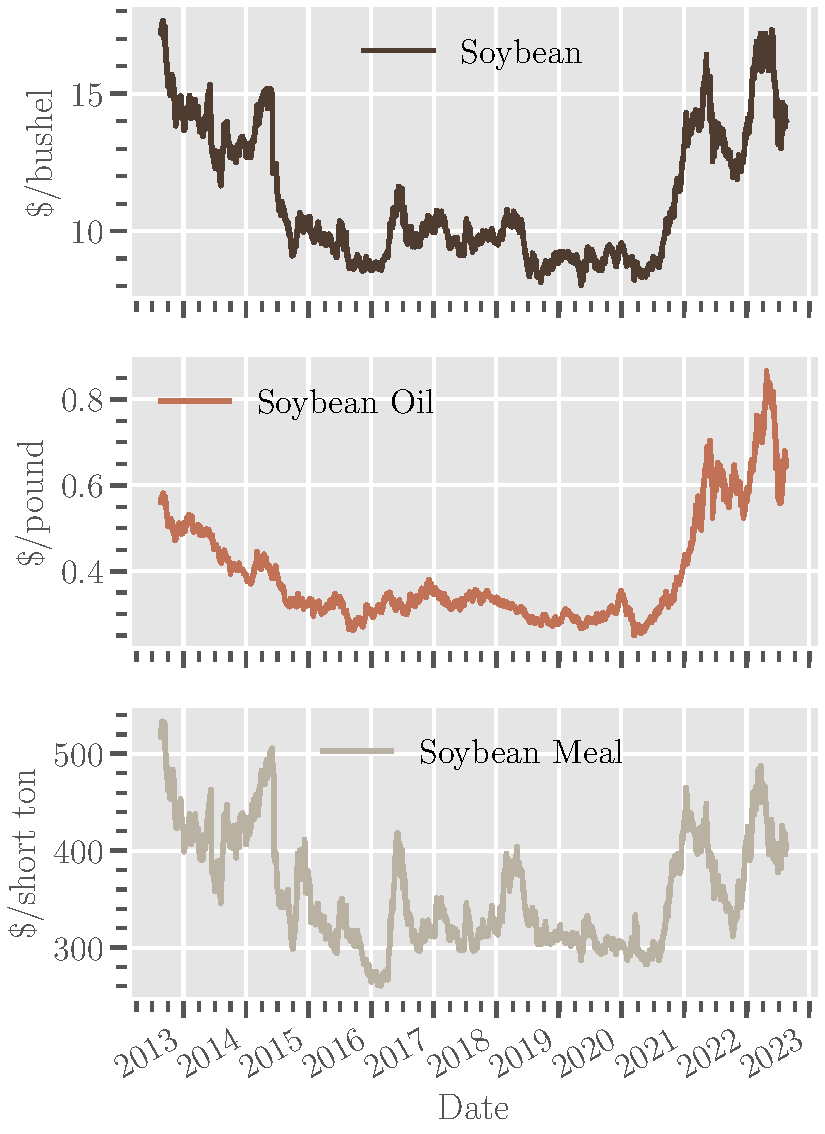
\includegraphics[width=\linewidth]{04_Original_Time_Series}
	\end{minipage}
	\begin{minipage}{0.45\linewidth}
	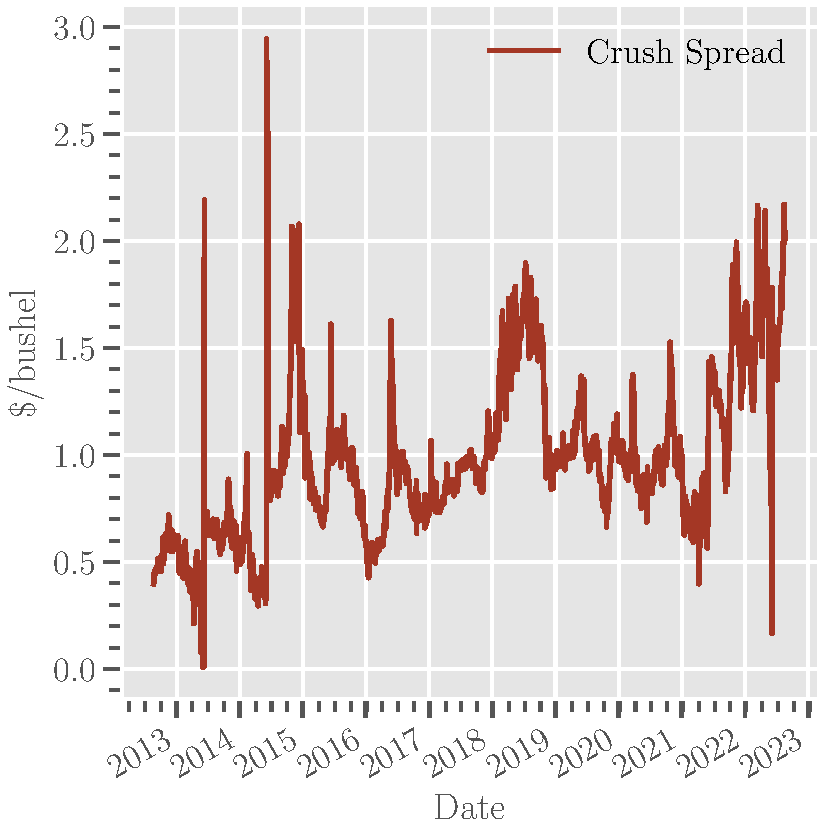
\includegraphics[width=\linewidth]{04_Spread_Series}
	\end{minipage}
	\caption{\textbf{Szeregi czasowe cen spot}. Lewy panel od góry: soja, olej sojowy, śruta sojowa. Prawy panel: 1-1-1 crush spread. \label{fig:original_time_series}}
\end{figure}

Szeregi czasowe były kompletne, poza wyjątkiem trzech obserwacji usuniętych manualnie z szeregu śruty sojowej. Użyliśmy strategii \emph{forward-fill}, aby uzupełnić tę lukę w danych przy pomocą ostatniej dostepnej wartości. Ponieważ soybean crush spreadem najczęściej handluje się w horyzontach miesięcy, zdecydowaliśmy, że modelowanie na dziennych przyrostach wartości nie będzie dobrym wyborem. Wszystkie szeregi zostały przekształcone do częstotliwości tygodniowej, poprzez wzięcie ostatniej dostępnej wartości w danym tygodniu, na podstawie czego policzyliśmy następnie logarytmiczne stopy zwrotu zgodnie z równaniem \ref{eq:logreturn}.

\emph{Exploratory data analysis} (EDA) rozpoczęliśmy od struktury zależności logarytmicznych stóp zwrotu, rysując wykresy punktowe widoczne na rysunku \ref{fig:pairplot_original_scale}. Widzimy na nich wysoki stopień zależności między komponentami spreadu, chociaż relacja samego spreadu z poszczególnymi z nich nie wydaje się być oczywista.

\begin{figure}[h]
	\centering
	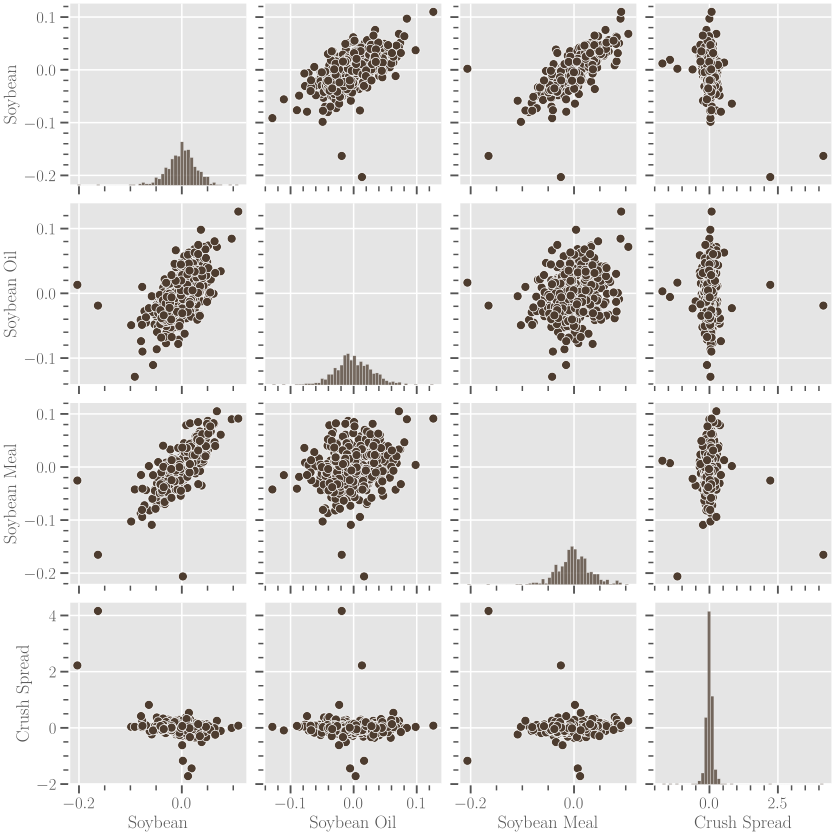
\includegraphics[width=0.9\linewidth]{04_PairPlot}
	\caption{\textbf{Wykresy zależności logarytmicznych stóp zwrotu.} Wykresy punktowe każdy-z-każdym, oraz histogramy wszystkich zmiennych. \label{fig:pairplot_original_scale}}
\end{figure}

Następnie zbadaliśmy ogony rozkładów logarytmicznych stóp zwrotu, kalibrując do nich rozkład normalny i porównując gęstości, oraz wykres ogonu w skali logarytmicznej. Rysunek \ref{fig:tail_analysis}, a szczególnie ich prawe panele wskazują na ciężkoogonowość, która uwydatniona jest najbardziej dla samego crush spreadu.\\

\begin{figure}[h]
	\centering
	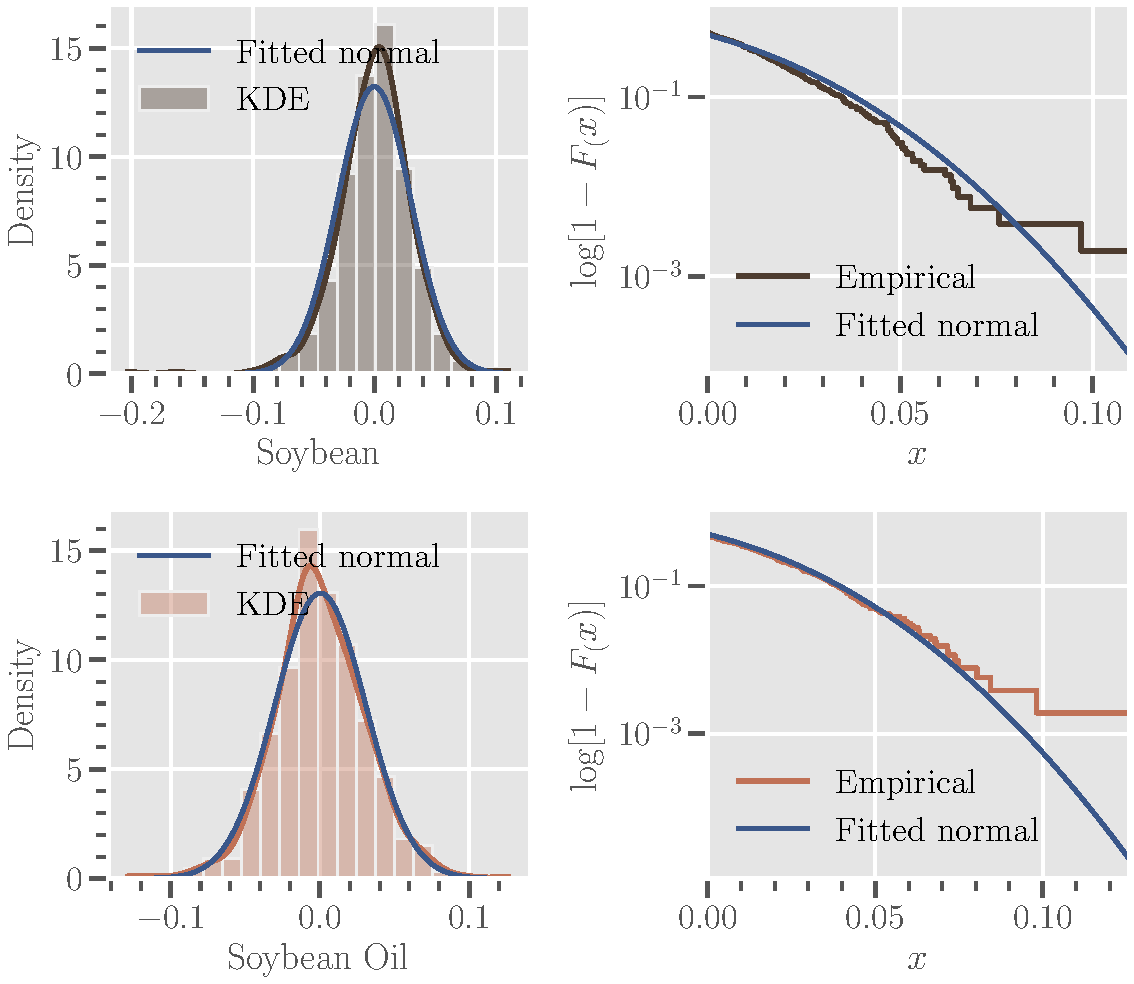
\includegraphics[width=0.7\linewidth]{04_TailAnalysis_1}
	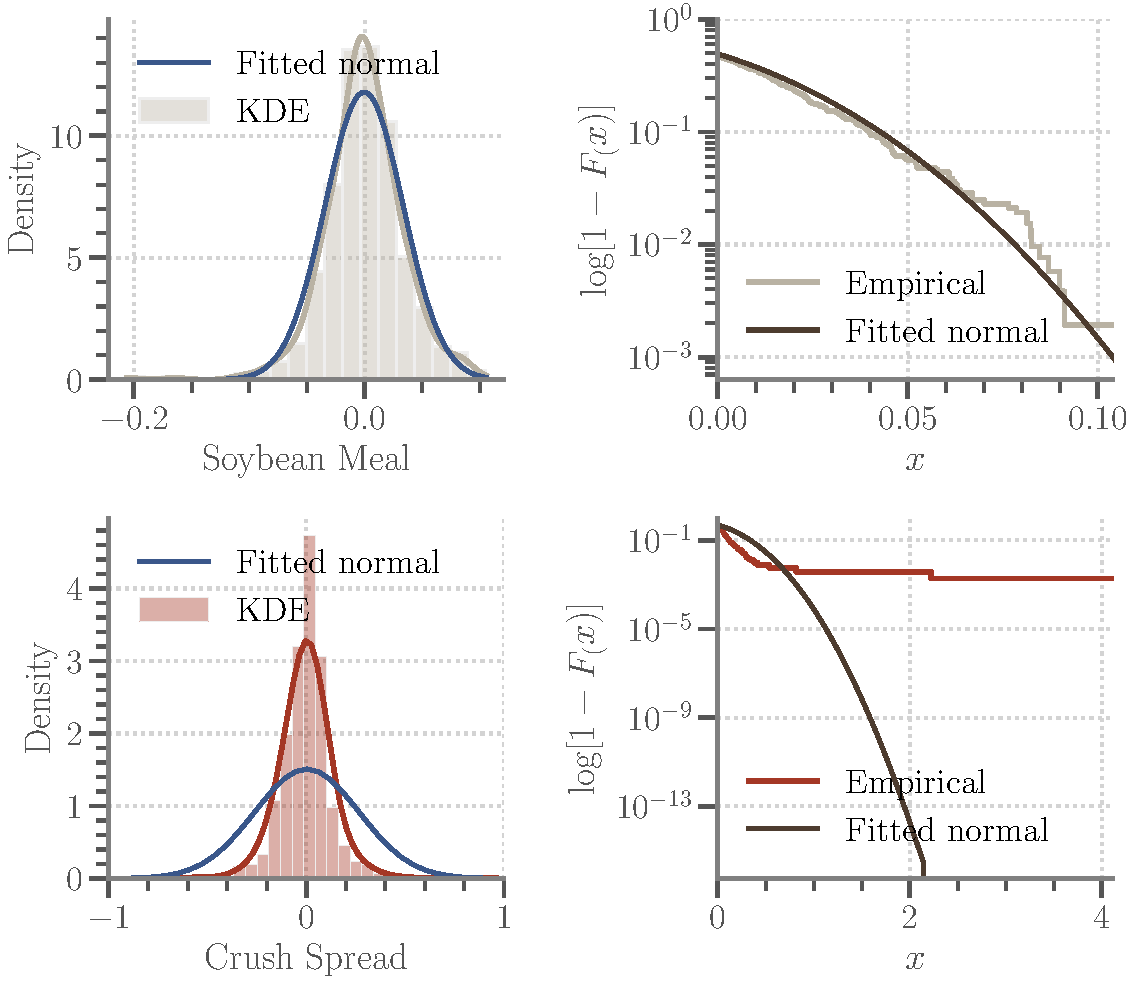
\includegraphics[width=0.7\linewidth]{04_TailAnalysis_2}
	
	\caption{\textbf{Ogony logarytmicznych stóp zwrotu.} Histogramy oraz \emph{kde} gęstości dla każdego aktywa, wraz z dopasowaną gęstością rozkładu normalnego (lewy panel). Empiryczny ogon danych w skali logarytmicznej, wraz z ogonem dopasowanego rozkładu normalnego (prawy panel). \label{fig:tail_analysis}}
\end{figure}

\FloatBarrier